\documentclass[10pt, handout]{beamer}
\usepackage[utf8]{inputenc}
\usepackage[T1]{fontenc}
\usepackage[french]{babel}
\usepackage{amsmath,amsfonts,amssymb}
\usepackage{graphicx}
\usepackage{algorithm}
\usepackage{algorithmicx}
\usepackage{algpseudocode}

% Theme configuration
\usetheme{Metropolis}
\usecolortheme{default}
\setbeamertemplate{navigation symbols}{}
\setbeamertemplate{footline}[frame number]

% Title information
\title{Exploration de la Recherche avec Tabous}
\subtitle{Métaheuristiques}
\author{Pierre BOURGEY, Paul BOUTET, Florian GIURGIU}
\institute{Télécom Saint-Etienne}
\date{9 mai 2025}

\begin{document}

% Title slide
\begin{frame}
    \titlepage
\end{frame}

% Table of contents
\begin{frame}{Plan}
    % Show only sections, not subsections
    \setbeamertemplate{section in toc}{\inserttocsection\par}
    \tableofcontents[hideallsubsections]
\end{frame}

\section{Introduction}
\subsection{Contexte Historique}
\begin{frame}{Contexte Historique}
    \begin{enumerate}
        \item Développement des métaheuristiques dans les années 1980
        \item Introduction de la recherche taboue par Fred Glover en 1986
        \item Applications dans divers domaines : optimisation, planification, etc.
    \end{enumerate}
\end{frame}

\subsection{Analogie Biologique}
\begin{frame}{Analogie Biologique}
    \begin{columns}[T] % Align columns at the top
        \begin{column}{0.33\textwidth}
            \textbf{Inspiration}
            \medskip

            Inspirée du comportement de recherche humain. \medskip

        \end{column}
        \begin{column}{0.33\textwidth}

            \textbf{Mécanisme}
            \medskip

            Un "tabou" similaire aux processus cognitifs. \medskip

        \end{column}
        \begin{column}{0.33\textwidth}
            \textbf{Stratégie}
            \medskip

            Évitement des mouvements déjà explorées.
            \medskip

        \end{column}
    \end{columns}
    \bigskip
    Cette approche s'inspire de la manière dont les humains explorent et évitent les erreurs.
\end{frame}

% Main content
\section{Principe Fondamental}
\subsection{Définitions}
\begin{frame}{Définitions}
    \begin{enumerate}
        \item \textbf{Voisinage} : Ensemble de solutions accessibles par un mouvement.
        \item \textbf{Mouvement} : Opération qui modifie une solution pour en obtenir une nouvelle. On peut utiliser un vecteur de déplacement, une permutation etc...
        \item \textbf{Tabou} : Mouvements interdits pour éviter les cycles locaux.
        \item \textbf{Temps en mémoire courte / taille mémoire} : Durée pendant laquelle un mouvement est considéré tabou (souvent fixé proche de 10 itérations ou généré aléatoirement pour chaque élément ajouté en mémoire afin d'éviter les cycles).
    \end{enumerate}
\end{frame}

\subsection{Algorithme}
\begin{frame}{Principe Fondamental}

    \begin{columns}[T] % Align columns at the top
        \begin{column}{0.6\textwidth}
            \raggedright
            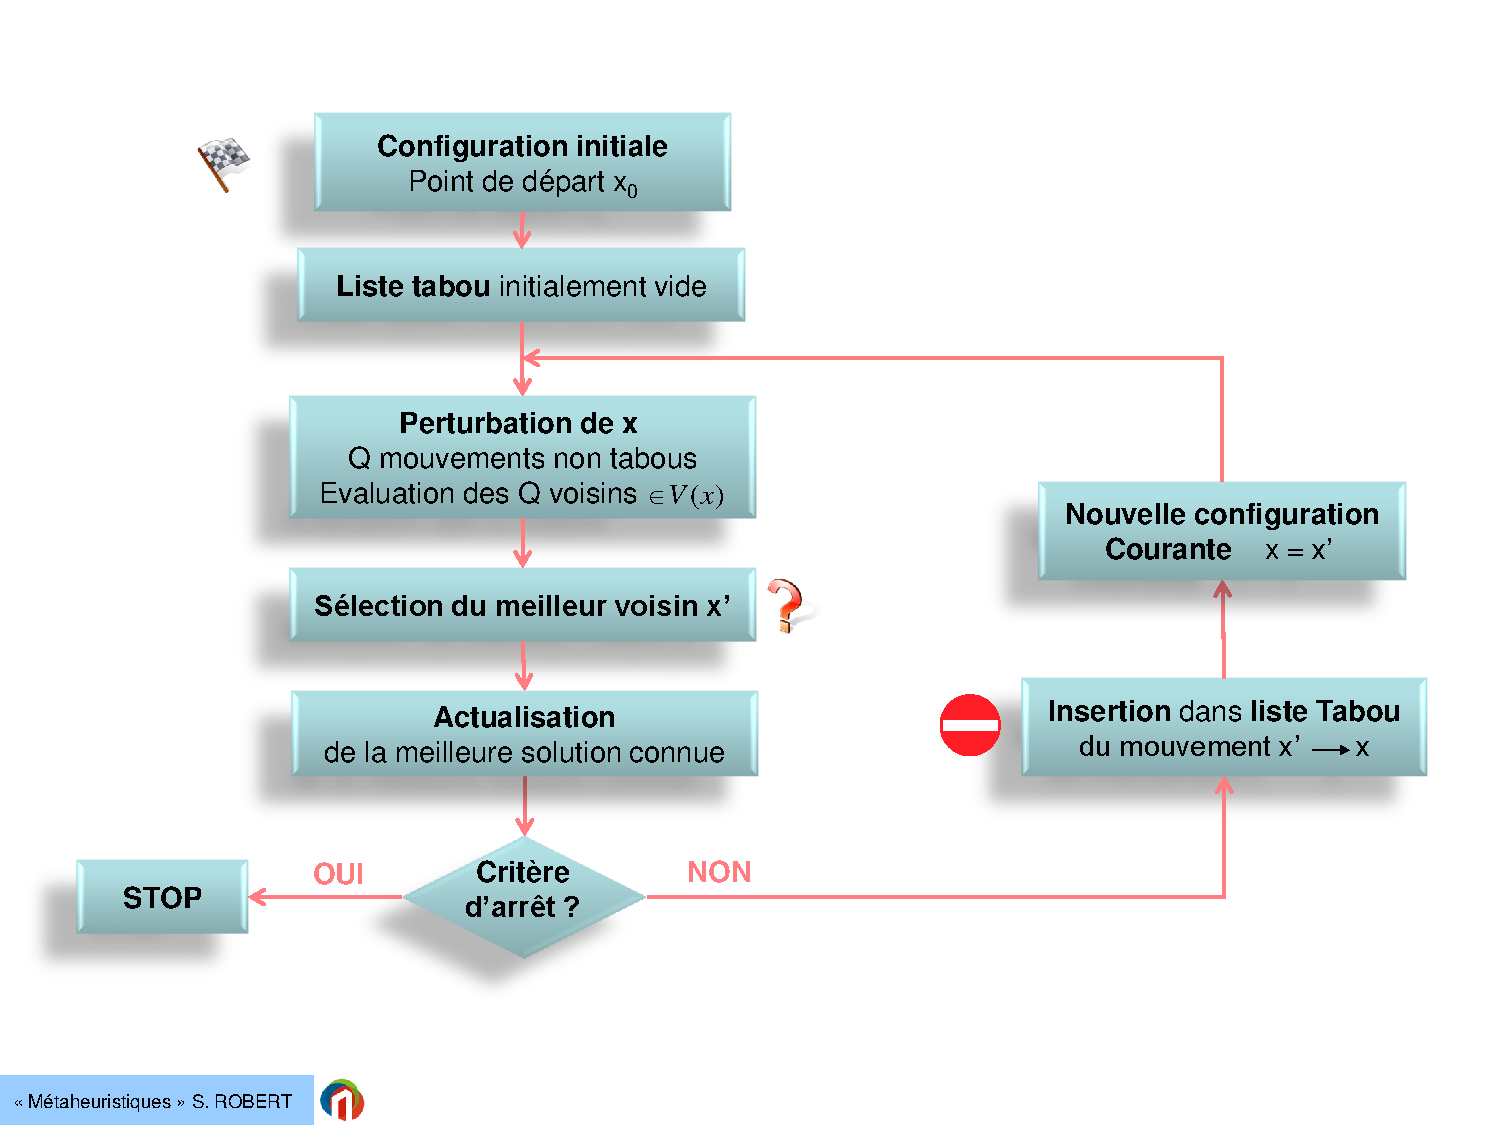
\includegraphics[width=7cm]{Docs_RT1.pdf}
        \end{column}

        \begin{column}{0.4\textwidth}

            \textbf{Exploration}
            \medskip

            Exploration systématique de l'espace de recherche. \medskip

            \textbf{Mémoire}
            \medskip

            Mécanisme de "mémoire courte" pour éviter les répétitions. \medskip

            \textbf{Évasion}
            \medskip

            Capacité de sortir des minima locaux.

        \end{column}
    \end{columns}
\end{frame}

\section{Extensions}
\subsection{Critère d'aspiration}
\begin{frame}{Critère d'aspiration}
    \textbf{Définition :} Le critère d'aspiration permet de contourner les mouvements tabous si une solution est suffisamment prometteuse. Cela évite de rester bloqué dans des minima locaux.

    \begin{exampleblock}{Exemple :}
        \begin{enumerate}
            \item Considérons des permutations où les mouvements sont des inversions de deux
                  éléments.
            \item Départ : \textbf{[1,2,3,4,5]} (coût : 3).
            \item Permutation : \textbf{[2,1,3,4,5]} (coût : 3), interdit \textbf{1
                      $\leftrightarrow$ 2}.
            \item Permutation : \textbf{[2,1,4,3,5]} (coût : 3), interdit \textbf{3
                      $\leftrightarrow$ 4}.
            \item Permutation : \textbf{[2,1,4,5,3]} (coût : 3), interdit \textbf{3
                      $\leftrightarrow$ 5}.
            \item Une meilleure solution \textbf{[1,2,4,5,3]} (coût : 2) existe, mais le
                  mouvement \textbf{1 $\leftrightarrow$ 2} est interdit.
            \item On effectue ce mouvement interdit car il améliore le coût global.
        \end{enumerate}
    \end{exampleblock}
\end{frame}

\subsection{Mémoire à long terme}
\begin{frame}{Mémoire à long terme}
    \textbf{Définition :} 
    La mémoire à long terme permet de garder une trace des mouvements qui ont été bénéfiques ou nuisibles dans le passé. Cela aide à éviter les mouvements qui ont conduit à mauvaises solutions.
    
    \bigskip

    \begin{exampleblock}{Exemple :}
        \begin{enumerate}
            \item Considérons un problème d'ordonnancement où certaines tâches sont plus
                  difficiles que d'autres.
            \item Un mouvement qui a conduit à une solution de mauvaise qualité dans le passé
                  sera évité dans le futur.
        \end{enumerate}
    \end{exampleblock}
    \bigskip
    \textbf{Avantages :}
    \begin{enumerate}
        \item Amélioration de la qualité des solutions trouvées.
        \item Réduction du temps de calcul en évitant les mouvements nuisibles.
    \end{enumerate}
\end{frame}

\subsection{Pénalisation des mouvements récurrents}
\begin{frame}{Pénalisation des mouvements récurrents}
    \textbf{Définition :} 
    La pénalisation des mouvements récurrents consiste à attribuer un coût plus élevé aux mouvements qui ont été effectués plusieurs fois dans le passé. Cela aide à éviter les cycles et à encourager l'exploration de nouvelles solutions.

    \bigskip

    \begin{exampleblock}{Exemple}
        \begin{enumerate}
            \item Considérons un problème de voyageur de commerce où certaines villes sont
                  visitées plusieurs fois.
            \item Un mouvement qui revient à une ville déjà visitée sera pénalisé.
        \end{enumerate}
    \end{exampleblock}
    \bigskip
    \textbf{Avantages :}
    \begin{enumerate}
        \item Encouragement de l'exploration de nouvelles solutions.
        \item Évitement des cycles et des solutions sous-optimales.
    \end{enumerate}
\end{frame}

\subsection{Extension des voisinages}
\begin{frame}{Extension des voisinages}
    \textbf{Définition :} 
    L'extension des voisinages consiste à élargir l'ensemble des solutions candidates en considérant des mouvements plus complexes. Cela permet d'explorer de nouvelles régions de l'espace de recherche.
    
    \bigskip

    \begin{exampleblock}{Exemple}
        \begin{enumerate}
            \item Considérons un problème d'optimisation où les mouvements sont des permutations
                  de plusieurs éléments.
            \item Un mouvement qui échange plusieurs éléments sera considéré comme un voisinage.
        \end{enumerate}
    \end{exampleblock}
    \bigskip
    \textbf{Avantages :}
    \begin{enumerate}
        \item Exploration de nouvelles solutions potentiellement meilleures.
        \item Évitement des minima locaux en diversifiant les mouvements.
    \end{enumerate}
\end{frame}

\subsection{Hybridation avec d'autres méthodes}
\begin{frame}{Hybridation avec d'autres méthodes}
    \textbf{Définition :}
    L'hybridation consiste à combiner la recherche taboue avec d'autres méthodes d'optimisation pour améliorer les performances. Cela permet de tirer parti des forces de chaque méthode.

    \bigskip

    Pour plus d'informations, voir la référence \cite{ref1}.
\end{frame}

% Two columns layout
\section{Avantages - Inconvénients}

\begin{frame}{Avantages}
    \begin{enumerate}
        \item Rapidité d'exécution.
        \item Résultats de qualité acceptable.
        \item Paramétrage simple (peu de paramètres : taille mémoire, itérations max).
    \end{enumerate}
\end{frame}

\begin{frame}{Rapidité}
    \begin{columns}
        \begin{column}{0.6\textwidth}
            \begin{figure}[ht]
                \begin{center}
                    \begin{tabular}{cc}
                        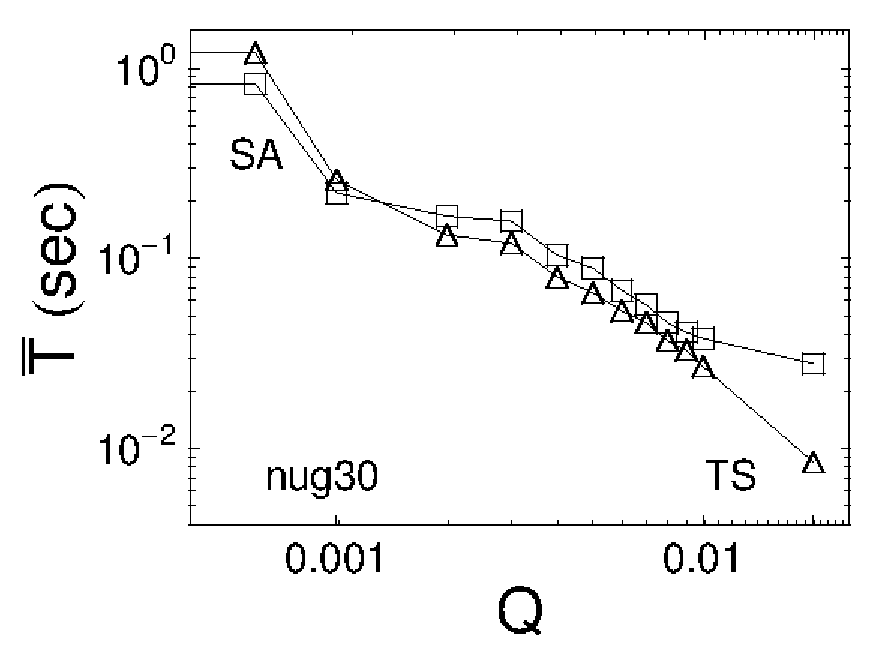
\includegraphics[width=2.2cm]{figures/pnug30Ro.eps}   &
                        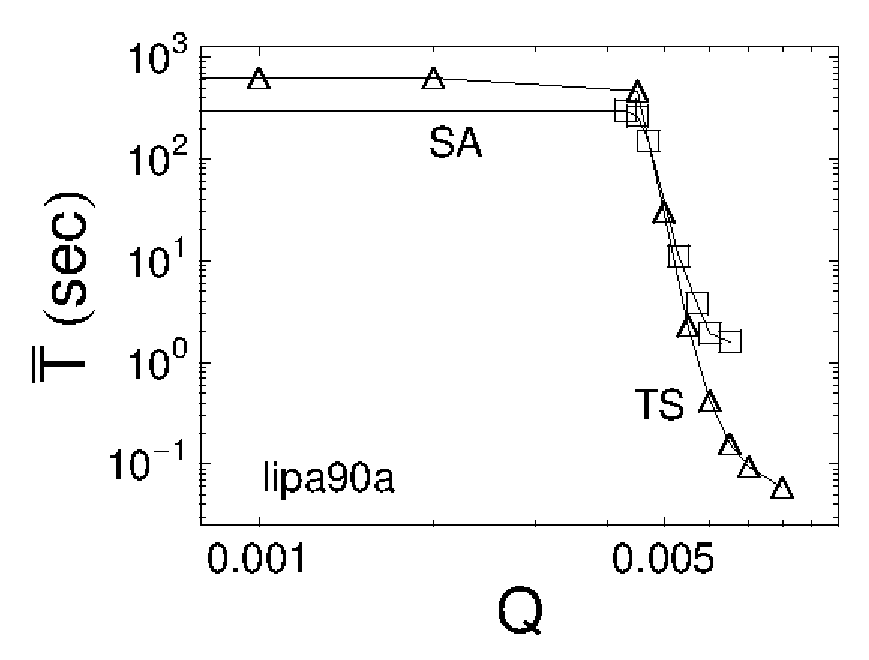
\includegraphics[width=2.2cm]{figures/plipa90aRo.eps}   \\
                        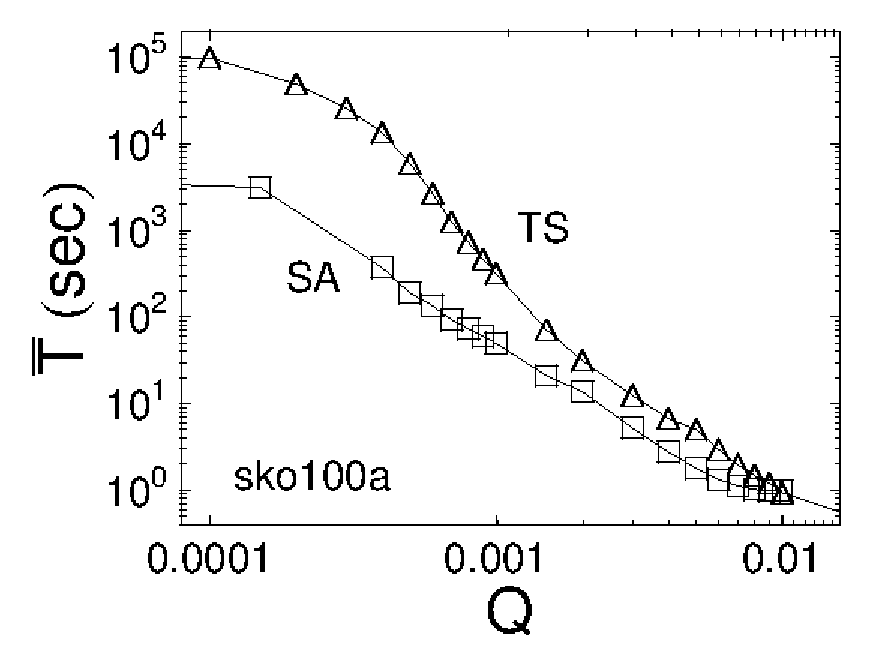
\includegraphics[width=2.2cm]{figures/psko100aRo.eps} &
                        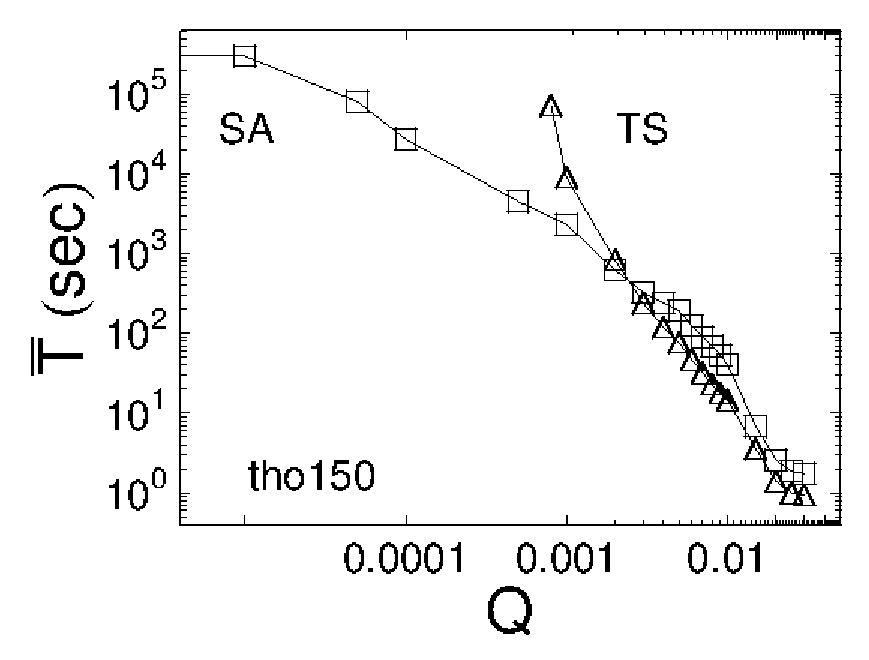
\includegraphics[width=2.2cm]{figures/ptho150Ro.eps}    \\
                        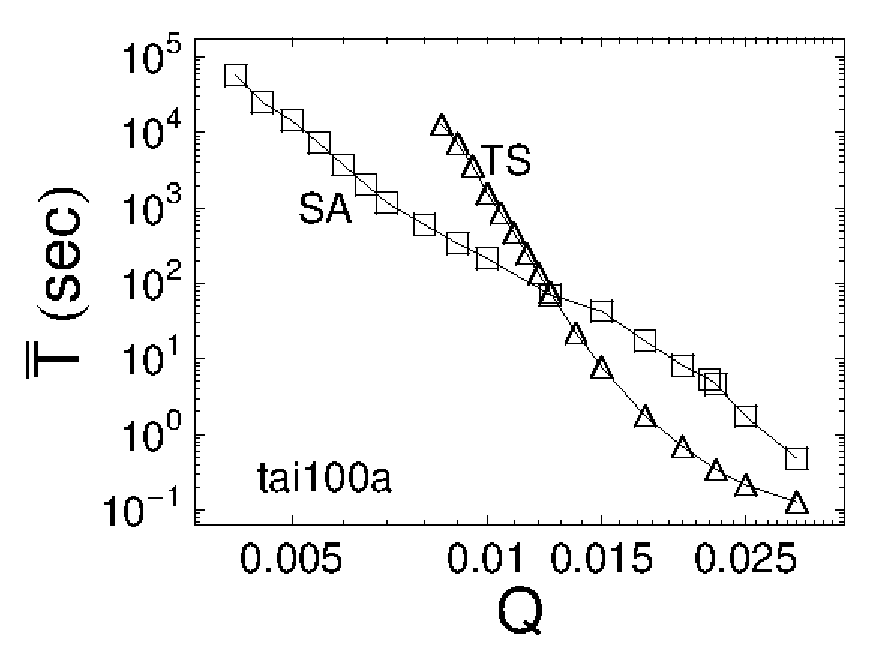
\includegraphics[width=2.2cm]{figures/ptai100aRo.eps} &
                        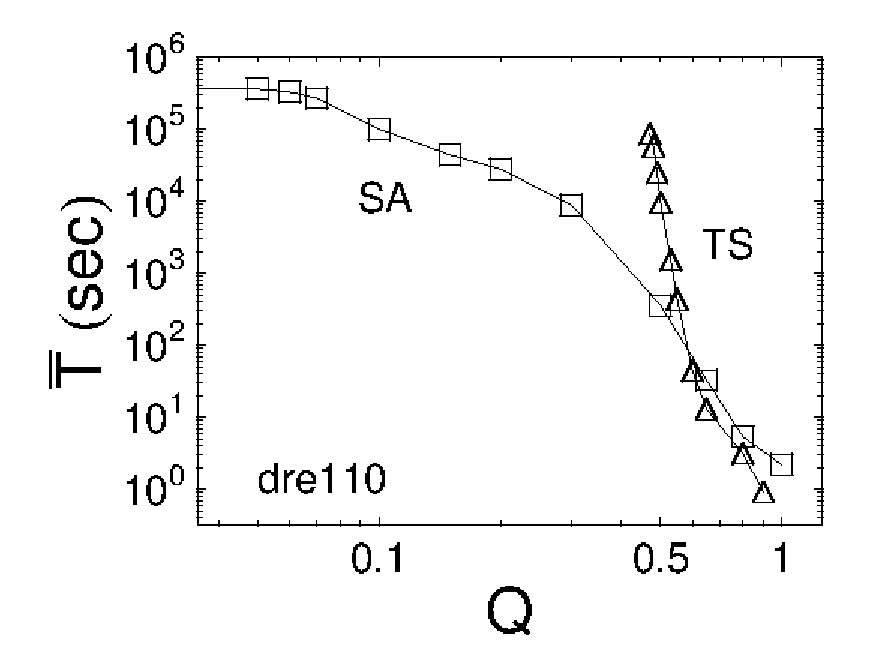
\includegraphics[width=2.2cm]{figures/pdre110Ro.eps}
                    \end{tabular}
                \end{center}
                \caption{$\bar T$ versus $Q$ for various problem instances for SA (squares) and TS (triangles).  For plots which
                    achieve the lowest known cost for an instance ($Q=0$), we extend the
                    line connecting the plot points to the left edge of the panel.}
                \label{pCRo}
            \end{figure}
        \end{column}
        \begin{column}{0.4\textwidth}

            \textbf{Mesures de performance:}
            \medskip

            $Q = \frac{C - C_{best}}{C_{best}}$ \\
            $C_{best}$ = meilleur coût connu \\
            $C$ = coût de la solution courante \\
            $\bar T$ = temps moyen pour atteindre une qualité Q.
        \end{column}
    \end{columns}
\end{frame}

\begin{frame}{Inconvénients}
    \begin{enumerate}
        \item Complexité de définition des mouvements et voisinages.
        \item Sensibilité aux paramètres (ex: taille de la mémoire, durée de la recherche).
    \end{enumerate}

\end{frame}

% Figure example
\section{Applications}

\begin{frame}{Problème d'Affectation Quadratique (QAP)}
    \framesubtitle{Formulation et enjeux}

    \begin{block}{Problématique centrale}
        Affecter \( n \) objets à \( n \) emplacements en minimisant :
        \[
            \sum_{i=1}^n \sum_{j=1}^n f_{ij} \cdot d_{p(i)p(j)}
        \]
        où :
        \begin{enumerate}
            \item \( f_{ij} \) : Flux entre l'objet \( i \) et \( j \) (non symétrique)
            \item \( d_{rs} \) : Distance entre l'emplacement \( r \) et \( s \) (symétrique)
            \item \( p(i) \) : Permutation donnant l'emplacement de l'objet \( i \)
        \end{enumerate}
    \end{block}

    \begin{exampleblock}{Défi algorithmique}
        \begin{enumerate}
            \item NP-difficile : Pas de solution exacte pour \( n > 20 \)
            \item Espace de solutions : \( n! \) permutations possibles
            \item Coût de calcul : \( \mathcal{O}(n^2) \) par évaluation
        \end{enumerate}
    \end{exampleblock}
\end{frame}

\begin{frame}{Problème d'Affectation Quadratique (QAP)}
    \begin{alertblock}{Applications réelles}
        \begin{columns}
            \column{0.45\textwidth}
            \begin{enumerate}
                \item Planification d'usine
                \item Placement de composants électroniques
                \item Optimisation de clavier
            \end{enumerate}

            \column{0.45\textwidth}
            \begin{enumerate}
                \item Répartition de fichiers
                \item Affectation de portes aéroportuaires
                \item Agencement hospitalier
            \end{enumerate}
        \end{columns}
    \end{alertblock}
\end{frame}

\begin{frame}{Exemple concret : Répartition de bâtiments}
    \framesubtitle{Cas d'étude avec 5 bâtiments et 5 emplacements}

    \begin{block}{Configuration du problème}
        \begin{enumerate}
            \item 5 bâtiments à placer sur 5 sites géographiques
            \item Objectif : Minimiser les déplacements entre bâtiments
            \item Deux matrices clés :
        \end{enumerate}
    \end{block}

    \begin{columns}[T]
        \column{0.45\textwidth}
        \begin{exampleblock}{Matrice des distances \(D\) (symétrique)}
            \[
                D = \begin{bmatrix}
                    0 & 1 & 2 & 3 & 1 \\
                    1 & 0 & 2 & 1 & 1 \\
                    2 & 2 & 0 & 1 & 2 \\
                    3 & 1 & 1 & 0 & 1 \\
                    1 & 1 & 2 & 1 & 0
                \end{bmatrix}
            \]
            \begin{footnotesize}
                \begin{center}
                    Distances en kilomètres
                \end{center}
            \end{footnotesize}
        \end{exampleblock}

        \column{0.45\textwidth}
        \begin{exampleblock}{Matrice des flots \(F\) (non symétrique)}
            \[
                F = \begin{bmatrix}
                    0 & 8 & 1 & 2 & 3 \\
                    5 & 0 & 2 & 1 & 2 \\
                    1 & 2 & 0 & 1 & 2 \\
                    2 & 1 & 1 & 0 & 6 \\
                    3 & 2 & 2 & 7 & 0
                \end{bmatrix}
            \]
            \begin{footnotesize}
                \begin{center}
                    Nombre de déplacements/jour
                \end{center}
            \end{footnotesize}
        \end{exampleblock}
    \end{columns}

\end{frame}

% --- Itération 0 ---
\begin{frame}{Itération 0 - Initialisation}
    \framesubtitle{Solution de départ}

    \begin{block}{Configuration initiale}
        \begin{enumerate}
            \item Permutation initiale : \( P = (2, 4, 1, 5, 3) \)
            \item Coût initial : 72
            \item Matrice de mémoire \( T \) vide
        \end{enumerate}
    \end{block}

    \begin{exampleblock}{Matrice d'interdiction initiale \( T \)}
        \[
            T = \begin{pmatrix}
                0 & 0 & 0 & 0 & 0 \\
                0 & 0 & 0 & 0 & 0 \\
                0 & 0 & 0 & 0 & 0 \\
                0 & 0 & 0 & 0 & 0 \\
                0 & 0 & 0 & 0 & 0
            \end{pmatrix}
        \]
    \end{exampleblock}
\end{frame}

% --- Itération 1 ---
\begin{frame}{Itération 1 }
    \framesubtitle{Exploration des voisins}

    \resizebox{\columnwidth}{!}{%
        \begin{tabular}{|c|c|c|c|c|c|c|c|c|c|c|}
            \hline
            Mouvement    & (1,2) & (1,3)        & (1,4)        & (1,5) & (2,3) & (2,4) & (2,5)        & (3,4) & (3,5) & (4,5) \\
            \hline
            \( \Delta \) & 2     & \textbf{-12} & \textbf{-12} & 2     & 0     & -10   & \textbf{-12} & 4     & 8     & 6     \\
            \hline
        \end{tabular}%
    }

    \begin{enumerate}
        \item 3 mouvements optimaux : \( \Delta = -12 \)
        \item Choix aléatoire : \( (1,3) \)
    \end{enumerate}

    \begin{columns}
        \column{0.5\textwidth}
        \begin{alertblock}{Nouvelle solution}
            \( P = (1, 4, 2, 5, 3) \) \\
            Coût : 60 \\
            \( t = 9 \) tiré aléatoirement
        \end{alertblock}

        \column{0.5\textwidth}
        \begin{exampleblock}{Mise à jour de \( T \)}
            \[
                T = \begin{pmatrix}
                    0  & 0 & 10 & 0 & 0 \\
                    10 & 0 & 0  & 0 & 0 \\
                    0  & 0 & 0  & 0 & 0 \\
                    0  & 0 & 0  & 0 & 0 \\
                    0  & 0 & 0  & 0 & 0
                \end{pmatrix}
            \]
        \end{exampleblock}
    \end{columns}
\end{frame}

% --- Itération 2 ---
\begin{frame}{Itération 2 }
    \framesubtitle{Gestion des interdictions}

    \resizebox{\columnwidth}{!}{%
        \begin{tabular}{|c|c|c|c|c|c|c|c|c|c|c|}
            \hline
            Mouvement    & (1,2) & (1,3)              & (1,4) & (1,5) & (2,3) & (2,4) & (2,5) & (3,4) & (3,5) & (4,5) \\
            \hline
            \( \Delta \) & 14    & \textcolor{red}{X} & 10    & 0     & 10    & 8     & 12    & 12    & 6     & -     \\
            \hline
        \end{tabular}%
    }

    \begin{enumerate}
        \item Mouvement \( (1,3) \) interdit (\( t_{13} = 10 \))
        \item Meilleur mouvement : \( (1,4) \) (\( \Delta = -8 \))
    \end{enumerate}

    \begin{columns}
        \column{0.5\textwidth}
        \begin{alertblock}{Nouvelle solution}
            \( P = (5, 4, 2, 1, 3) \) \\
            Coût : 52 \\
            \( t = 6 \) tiré aléatoirement
        \end{alertblock}

        \column{0.5\textwidth}
        \begin{exampleblock}{Mise à jour de \( T \)}
            \[
                T = \begin{pmatrix}
                    8  & 0 & 10 & 0 & 0 \\
                    10 & 0 & 0  & 0 & 0 \\
                    0  & 0 & 0  & 0 & 0 \\
                    0  & 0 & 0  & 0 & 0 \\
                    0  & 0 & 0  & 8 & 0
                \end{pmatrix}
            \]
        \end{exampleblock}
    \end{columns}
\end{frame}

% --- Itération 3 ---
\begin{frame}{Itération 3}
    \framesubtitle{Stratégie de diversification}

    \resizebox{\columnwidth}{!}{%
        \begin{tabular}{|c|c|c|c|c|c|c|c|c|c|c|}
            \hline
            Mouvement    & (1,2) & (1,3) & (1,4) & (1,5) & (2,3) & (2,4) & (2,5) & (3,4) & (3,5) & (4,5) \\
            \hline
            \( \Delta \) & 10    & 24    & 10    & 0     & 22    & 20    & 8     & 8     & 14    & -     \\
            \hline
        \end{tabular}%
    }

    \begin{enumerate}
        \item Aucun \( \Delta < 0 \) (minimum local)
        \item Choix du moins mauvais : \( (2,3) \) (\( \Delta = +8 \))
    \end{enumerate}

    \begin{columns}
        \column{0.5\textwidth}
        \begin{alertblock}{Nouvelle solution}
            \( P = (5, 2, 4, 1, 3) \) \\
            Coût : 52 \\
            \( t = 8 \) tiré aléatoirement
        \end{alertblock}

        \column{0.5\textwidth}
        \begin{exampleblock}{Mise à jour de \( T \)}
            \[
                T = \begin{pmatrix}
                    8  & 0  & 10 & 0 & 0 \\
                    10 & 0  & 11 & 0 & 0 \\
                    0  & 0  & 0  & 0 & 0 \\
                    0  & 11 & 0  & 0 & 0 \\
                    0  & 0  & 0  & 8 & 0
                \end{pmatrix}
            \]
        \end{exampleblock}
    \end{columns}
\end{frame}

% --- Itération 4 ---
\begin{frame}{Itération 4}
    \framesubtitle{Convergence}

    \resizebox{\columnwidth}{!}{%
        \begin{tabular}{|c|c|c|c|c|c|c|c|c|c|c|}
            \hline
            Mouvement    & (1,2) & (1,3) & (1,4) & (1,5) & (2,3) & (2,4) & (2,5) & (3,4) & (3,5) & (4,5) \\
            \hline
            \( \Delta \) & 24    & 10    & 10    & 8     & 8     & 22    & 20    & 14    & -     & -     \\
            \hline
        \end{tabular}%
    }

    \begin{enumerate}
        \item Mouvement \( (2,4) \) choisi (\( \Delta = +8 \))
    \end{enumerate}

    \begin{columns}
        \column{0.5\textwidth}
        \begin{alertblock}{Nouvelle solution}
            \( P = (5, 1, 4, 2, 3) \) \\
            Coût : 60 \\
            \( t = 5 \) tiré aléatoirement
        \end{alertblock}

        \column{0.5\textwidth}
        \begin{exampleblock}{Mise à jour de \( T \)}
            \[
                T = \begin{pmatrix}
                    8  & 0  & 10 & 9 & 0 \\
                    10 & 9  & 11 & 0 & 0 \\
                    0  & 0  & 0  & 0 & 0 \\
                    0  & 11 & 0  & 0 & 0 \\
                    0  & 0  & 0  & 8 & 0
                \end{pmatrix}
            \]
        \end{exampleblock}
    \end{columns}
\end{frame}

% --- Itération 5 ---
\begin{frame}{Itération 5}
    \framesubtitle{Contournement des interdictions}

    \resizebox{\columnwidth}{!}{%
        \begin{tabular}{|c|c|c|c|c|c|c|c|c|c|c|}
            \hline
            Mouvement    & (1,2) & (1,3)        & (1,4)               & (1,5) & (2,3)               & (2,4)               & (2,5) & (3,4) & (3,5) & (4,5) \\
            \hline
            \( \Delta \) & 12    & \textbf{-10} & \textcolor{gray}{X} & 10    & \textcolor{gray}{X} & \textcolor{gray}{X} & 4     & 14    & 20    & 10    \\
            \hline
        \end{tabular}%
    }

    \begin{enumerate}
        \item 1 mouvement optimal : \( (1,3) \) (\( \Delta = -10 \))
        \item Mouvements \( (1,4) \), \( (2,3) \), \( (2,4) \) interdits
    \end{enumerate}

    \begin{columns}
        \column{0.5\textwidth}
        \begin{alertblock}{Nouvelle solution}
            \( P = (4, 1, 5, 2, 3) \) \\
            Coût : 50 \\
            \( t = 6 \) tiré aléatoirement
        \end{alertblock}

        \column{0.5\textwidth}
        \begin{exampleblock}{Mise à jour de \( T \)}
            \[
                T = \begin{pmatrix}
                    8  & 0  & 10 & 9 & 0 \\
                    10 & 9  & 11 & 0 & 0 \\
                    0  & 0  & 0  & 0 & 0 \\
                    0  & 11 & 11 & 0 & 0 \\
                    11 & 0  & 0  & 8 & 0
                \end{pmatrix}
            \]
            \begin{enumerate}
                \item Interdiction : \( (4,3) \) et \( (5,1) \) jusqu'à itération 11
            \end{enumerate}
        \end{exampleblock}
    \end{columns}
\end{frame}

% References
\begin{frame}{Références}
    \begin{thebibliography}{9}
        \bibitem{ref1} Jebari H. - Rahali El Azzouzi S. - Samadi H. (2016). \textit{Hybridation des métaheuristiques pour la résolution de problème d’ordonnancement multi-objectif dans un atelier flow-shop}.
        \bibitem{ref2} Gerald Paul, (2010). \textit{Comparative Performance of Tabu Search and Simulated Annealing Heuristics for the Quadratic Assignment Problem}.
    \end{thebibliography}
\end{frame}

\end{document}